
We show our implementation in this section, including testbed setting, the whole workflow and implementation result such as code lines and FPGA resource consumption. We implement our design based on Xilinx official example of Ethernet 10/25G system.
\subsection{Testbed Configuration}
We implement our NAT with AMD (Xilinx) Zynq UltraScale+ MPSoC ZCU102 (called the board later). The evaluation setup includes the board, a router and a desktop machine.
We run a Linux \todo{Version} on the four PS ARM cores of the board. 
The desktop runs Ubuntu 18.04 equipped with a Nvidia (Mellanox) ConnectX-3 
with driver version \todo{??} whose line rate is 10Gbps. The MTU is configured as 9000B.
The performance of router is not critical since we only use it to ssh connect to the board.

\textbf{Network Topology.} 
The board and the on-board NIC of desktop are both connected to the router and 
are configured under the same subnet. 
For data plane, we connect the SPF interface of the board and a interface of ConnectX-3 back-to-back to fully investigate the potential of our FPGA NAT.

\subsection{Implementation Workflow}

We elaborate our detailed implementation workflow, which includes Verilog design and testing, Vivado block design, Petalinux image building, testbed deployment and Vitis cross-compile in this subsection. We use Vivado 19.02, Vitis 19.02, and Petalinux 19.02. Figure 1 shows our workflow.

\textbf{Hardware implementation and testing.} We use Verilog to implement our design in about 300 lines of code. We use Verilator to test the correctness of our implementation.
The testing code is about 1.5k lines in C++.

\textbf{Vivado block design and synthesis.} We use Vivado to insert our Verilog implementation as custom IPs, and then synthesis, implement, and generate bitstream. Finally we export the hardware to an \verb|.xsa| file. The delta of resource consumption between the original example and our modified design is \todo{????????}. 
% Note that ConnectX-3 has the feature of L2, L3, and L4 checksum offloading. 
% We cannot disable it directly due to driver bugs.
Note that we use a custom Ethernet protocol number rather than \verb|0x0800| to prevent potential complexities such as NIC checksum-offloading and Linux kernel sanity check. Therefore, we do not need to insert CSU IP.

\textbf{Petalinux image building.} Petalinux is a tool to build tiny embedded linux images.
The built image can be placed into an SD card to boot up the whole board. 
We build the images following the official tutorial in a Ubuntu 18.04 docker container over AMD Ryzen 7 7700 (4.8Ghz full core). It takes up to several hours.

\textbf{Vitis cross-compilation.} We need to cross-compile the C++ source code since the CPUs on the board are ARM core. We do it via Vitis, and scp the generated ELF file to the board directly.




\begin{figure*}[ht]
    \centering
    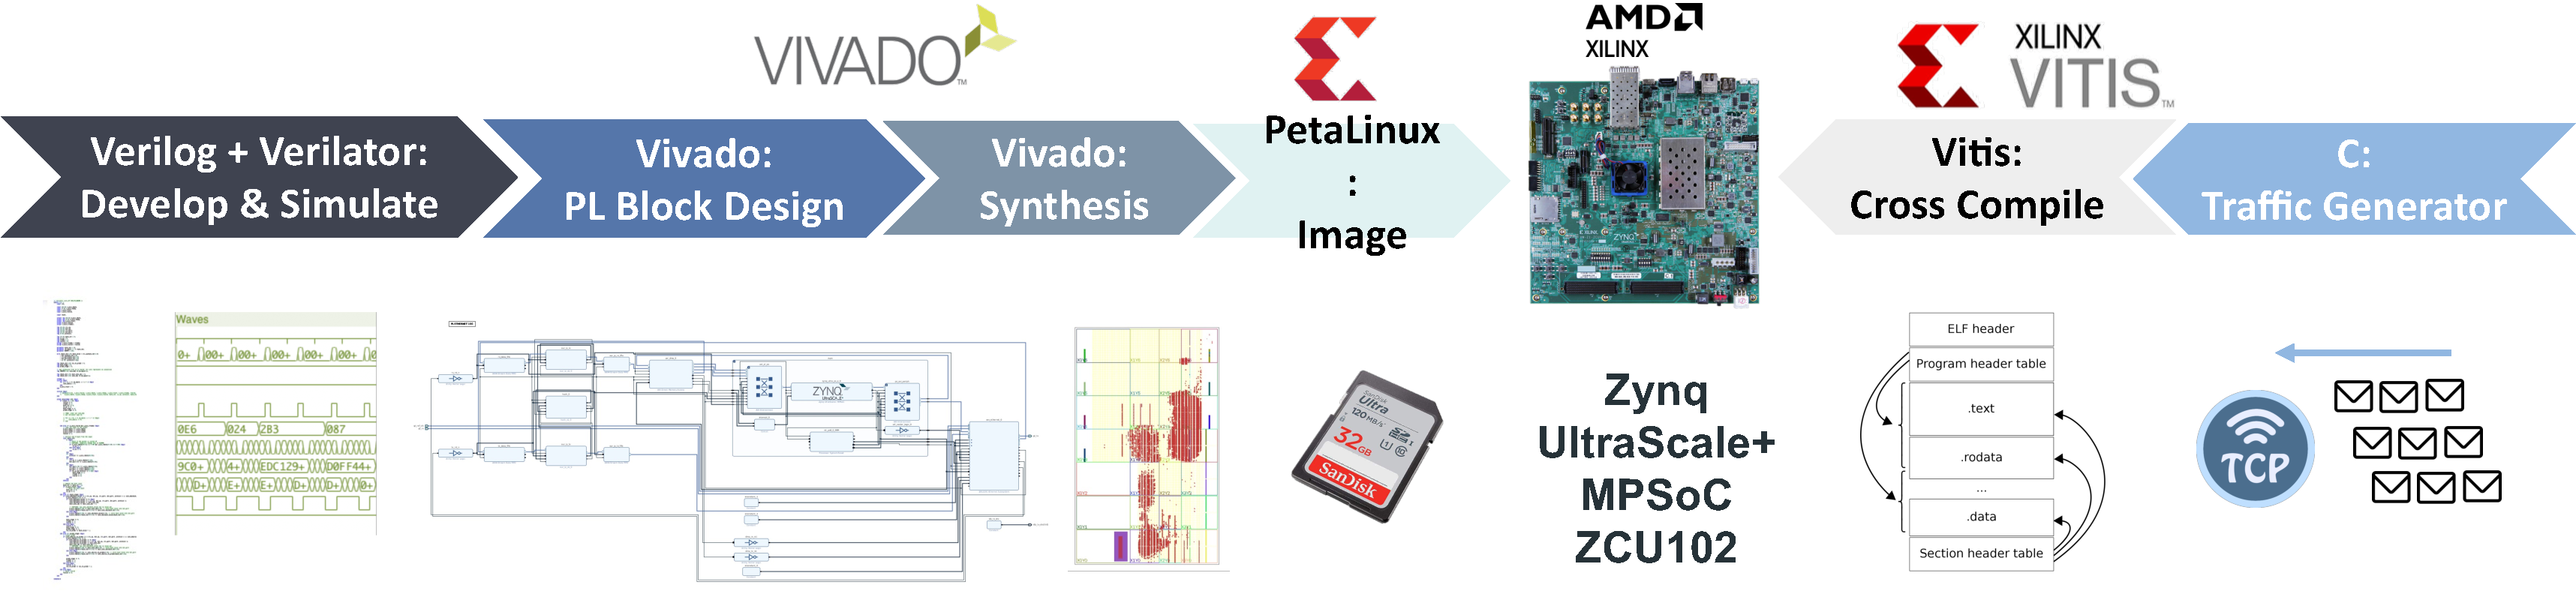
\includegraphics[width=500pt]{images/implworkflow.pdf}
    \caption{Our implementation workflow. }
\end{figure*}


% ○FPGA型号
% ○网络拓扑
% ○workflow,以及所有工具的版本
% ○soarx以及fpga上驱动版本号
% ○soarx、fpga上的Linux发行版以及内核版本
% ○网卡型号光纤线?光模组
% ○FPGA综合后占的资源
% ○代码行数
% ○
% ○表大小1024,MTU9000
% ○因为用了不同协议号,所以不需要插入CSU IP
% ○Detailed setting
